\chapter{Bijlagen}

\section{Opmerkingen cryptografisch expert}
\label{sec:opmerkingen-cryptografisch-expert}

"Dit bleek uiterst gevaarlijk toen de NSA een met opzet gebrekkige random
number generator publiceerde genaamd Dual\_EC\_DRBG. -> referentie nodig.
Daarnaast zou je hierover ook eventueel nog iets kunnen zeggen:
\url{http://www.reuters.com/article/us-usa-security-rsa-idUSBRE9BJ1C220131220}

I.v.m. keysterkte, RNG, hashing, kan je met volgende referentie ook helpen:
\url{http://dx.doi.org/10.6028/NIST.SP.800-131Ar1}

Je punt van snelheidsverlies tegenover securitywinst komt duidelijk over. Je
kan echter best wel vermelden welke hardware (op zijn minst het model van de
CPU en het type RAM vermelden) je bij de metingen gebruikt hebt. Dat kan een
rol spelen in verband van reproduceerbaarheid van de resultaten. Tevens ook
vermelden of je een VM gebruikt hebt. VMs hebben namelijk typisch een slechtere
performance op vlak van crypto dan echte hardware.

Ik mis op het einde nog een stukje conclusie m.b.t. de grootte van de sleutels
die je wil gaan gebruiken. Bij \ref{sec:gebruikte-algoritmes} gaf je duidlijk
aan dat "We kunnen  concluderen dat tot ECC-implementaties verder uitgewerkt en
gestandaardiseerd zijn, het best is om RSA te gebruiken.". Zoiets zou hier ook
meerwaarde hebben. Zie bijvoorbeeld opensslspeedtest.txt, waar mijn oude Intel
Core 2 Duo FTPServer het opneemt tegen een mijn Intel Xeon VPS.

Inleiding: hier zou je nog kunnen bijschrijven waarom key distribution zo
kritisch is (MitM natuurlijk).
Inleiding: "Om te zorgen dat elke nieuwe werknemer niet moet persoonlijk zich
identificeren met elke andere werknemer [...]". Ik weet wel dat dat een gevolg
zou zijn van de keuze die je gemaakt hebt voor Web Of Trust, maar dat is voor
de lezer niet direct duidelijk. Ik zou het er expliciet bijzetten.

\subsection{\fullref{subsec:aankomst-nieuwe-werknemer}}

Ik zou hier ook even een kort overzichtje geven met de stappen waardoor een
nieuwe werknemen zal moeten gaan:
1. Keypair genereren;
2. Centrale public key tekenen;
3. Eigen public key naar de server verzenden.

Tim zijn sleutel moet nog gevalideerd worden.  Vermeld erbij vanwaar de
centrale sleutel komt. Wie genereert hem? Waar staat hij opgeslagen? Hoe
verifiëren werknemers dat de cetnrale sleutel die zij op hun scherm zien de
juiste is? Welk medium is het meest betrouwbaar? USB? Misschien hangt de
publieke sleutel ergens op een prikbord? Of misschien kan internal IT de
sleutel mee voorinstalleren bij het prepareren van het werkstation van de
werknemer? Welk medium is praktisch het meest haalbaar? Welke afwegingen maak
je hierbij? Security vs convenience. Ongebruiksvriendelijke security is in de
echte wereld een reëel risico. Tegelijkertijd is gebruiksvriendelijke zwakke
security ook niet optimaal.

Geeft deze het juiste vertrouwensniveau -> Verwijs misschien ook naar hoofdstuk
6, voor meer informatie rond vertrouwensniveau's.

"Het proces dat zojuist werd beschreven waarin Tim de centrale sleutel(s)
importeert, kan automatisch gedaan worden door een intern programma." Tot op
zeker niveau wel. De publieke sleutel zal ofwel in de software ingebakken zijn
(in dat geval verifieert Tim best de hash van de software voor hij die
uitvoert), ofwel zal Tim de fingerprint manueel nog moeten ingeven/verifiëren.

"De publieke sleutel van Tim moet nu nog geïmporteerd worden in het netwerk van
het bedrijf en ondertekend worden door de centrale sleutel." Hierbij vermelden
waarom dat nog moet.

" Tim importeert zijn sleutel van de private keyserver [..]" -> Tim
importeert zijn *publieke* sleutel

Waarom moet Tim lokaal een kopie hebben van
zijn door de server ondertekende sleutel? Volgens mij is dat niet echt
noodzakelijk? Iemand die met Tim wil communiceren kan toch evengoed Tim's
sleutel van de private keyserver afhalen? Zal Tim altijd zijn USB stick moeten
bovenhalen om zijn sleutel te delen? Is het zo onredelijk dat een interne
private keyserver minder te vertrouwen dan een USB stick?

"Het is daarom een goed idee om twee USB-apparaten te maken." Het zou in
ieder geval nuttig zijn om een backup te voorzien. Misschien is het zelfs
handiger om het geëncrypteerde volume van de USB stick binnen het
bedrijfsnetwerk ergens te backuppen? Zo vermijd je de risico's en extra vereise
veiligheidsmaatregelen van de volgende subsection.

\subsection{\fullref{subsec:online-opslag-van-de-private-sleutel}}
"De cloud omgeving moet zero knowledge zijn." Een redelijk grote sprong
tussen dit en de vorige paragraaf. Je zou dat kunnen oplossen door iets hoger:
"private sleutel online op te slaan" -> "private sleutel online (i.e. cloud) op
te slaan". Druk "zero knowledge" best ook cursief.

De term "container" komt hier plotseling op de proppen en wordt vanaf dit
punt nog vaak gebruikt. Deze term heb je nergens geïntroduceerd. Daardoor
onstaat verwarring bij de lezer. Ik zou tussen de eerste en tweede paragraaf
een nieuw paragraafje (of twee) schrijven met wat uitleg in logische volgorde:
- Dat je plant om keypairs in de cloud op te slaan.
- Dat je hiervoor cloud zou kunnen gebruiken of eigen infrastructuur.
- Dat cloud eigenlijk toch wel gemakkelijk is omdat je dan zelf geen
infrastructuur moet aanleggen.
- Het kiezen voor cloud komt met bepaalde risico's: je moet de cloud provider
wel ten zeerste vertrouwen.
- Is er geen andere oplossing dan de cloudprovider te vertrouwen?
- Er bestaat zoiets als encrypted containers, die in principe doen wat Fig 7.2
uitbeeldt (bijv. VeraCrypt).
- Die encrypted containers zou je wel veilig in de cloud kunnen uploaden, mits
Zero Knowledge.
- Wat is zero knowledge?
-> De cloud omgeving moet zero knowledge zijn.

De term "hash" heb je ook nog niet geïntroduceerd. Mogelijk past er wel nog
een kort stukje over one-way functions en hashing in Hoofdstuk
\ref{ch:methodologie}? In dat geval
zou ik hier ook zeker naar H\ref{ch:methodologie} refereren. In dat stukje kan
je bijvoorbeeld de
belangrijkste eigenschappen van goeie hashing functies vermelden (met "voor
meer informatie <literatuur referentie>"). Alsook preimage resistance,
second-preimage resistance, collision attack,...

Merk ook op dat je best ook salt wanneer je hasht.


Ah, nu zie ik waarom je een tweede keer dacht te hashen langs de kant van de
server. Is m.i. nog steeds niet nodig hoor :-) Beschouw bijvoorbeeld een
succesvolle MitM. De aanvaller heeft in dit geval de username en H(p). Stel dat
hij erin slaagt om, op een voor de server legitieme wijze, de gebruikersnaam
van het slachtoffer en H(p) aan te bieden. Dan zal de server de versleutelde
container van de user terugsturen. En wat dan nog? Als H een goede hashing
functie is, en er gesalt is geweest, is de kans dat de aanvaller het wachtwoord
van de user kan berekenen astronomisch klein.
En dan nog... zelfs bij slechtere hashing functies is de kans nog steeds klein.
Beeld je bijvoorbeeld in dat we MD5 zouden gebruiken. De kans op een collision
is hierbij enorm groot. Maar, aangezien de container die je opslaat encrypted
is met AES, ben je met een collision niet veel.
Een voorbeeld: stel, ik versleutel mijn container met AES-128 en beveilig met
de passphrase "mysecretpassword". Veronderstel ook dat MD5("mysecretpassword")
= MD5("md5sucks"). Een aanvaller kan vinden dat MD5("md5sucks") dezelfde MD5
hash geeft als de hash die hij heeft afgeluisterd. Echter, geeft "md5sucks"
geen toegang tot de versleutelde container. Daarvoor heb je "mysecretpassword"
nodig.

Ik zou zeggen, hou beide verhalen in je paper! Wat je al hebt en wat ik hier
zojuist heb neergeschreven biedt zeker een toegevoegde waarde voor een
geïnteresseerde lezer!

Let wel, jouw voorbeeld met een extra hashing biedt geen extra beveiliging in
geval van MitM; enkel wanneer de aanvaller niet weet welke hash je serverside
gebruikt. Dat laatste als assumptie nemen, is tegen het Kerckhoffs principe.
Geen goed idee dus :-)

\subsection{\fullref{sec:wachtwoordsterkte}}
"Wachtwoordzinnen zijn een goede oplossing voor het onthouden van langere
wachtwoorden" -> [...], wat de XKCD comic ook aangeeft.

"Het laten vervallen van wachtwoorden is afgeraden[...]". Hier neem je een
minder conventionele stand in. Voor mij is dat ok, maar je stelt het toch best
iets genuanceerder. Het is nog altijd zo dat eens per 90-180 dagen veranderen
van wachtwoord aanbevolen is en technisch gezien extra beveiliging met zich
meebrengt. Daarentegen is het ook waar dat gebruikers echt niet elke 90-180
dagen moeite willen doen om wachtwoorden van 16 of meer karakters van buiten
leren, en er dan weggetjes rond gaan vinden, zoals je al schrijft. Indien ik de
beslissing moest maken, zou ik eens per jaar van wachtwoord veranderen een
acceptabel compromis vinden.

\subsection{\fullref{sec:verlies-wachtwoord-of-private-sleutel}}
"Om de werknemer verder te kunnen laten werken moeten de stappen van een
nieuwe werknemer opnieuw uitgevoerd worden." -> hier zou ik refereren naar
Sectie \ref{subsec:aankomst-nieuwe-werknemer}

"UTF-16 is 1 112 064" -> realistisch gezien gaan gebruikers maximum 95
verschillende karakters gebruiken (ascii tabel - controle characters), dwz
2\textasciicircum95 (ongeveer 4*10\textasciicircum28) mogelijkheden

\section{Bachelorproefvoorstel}
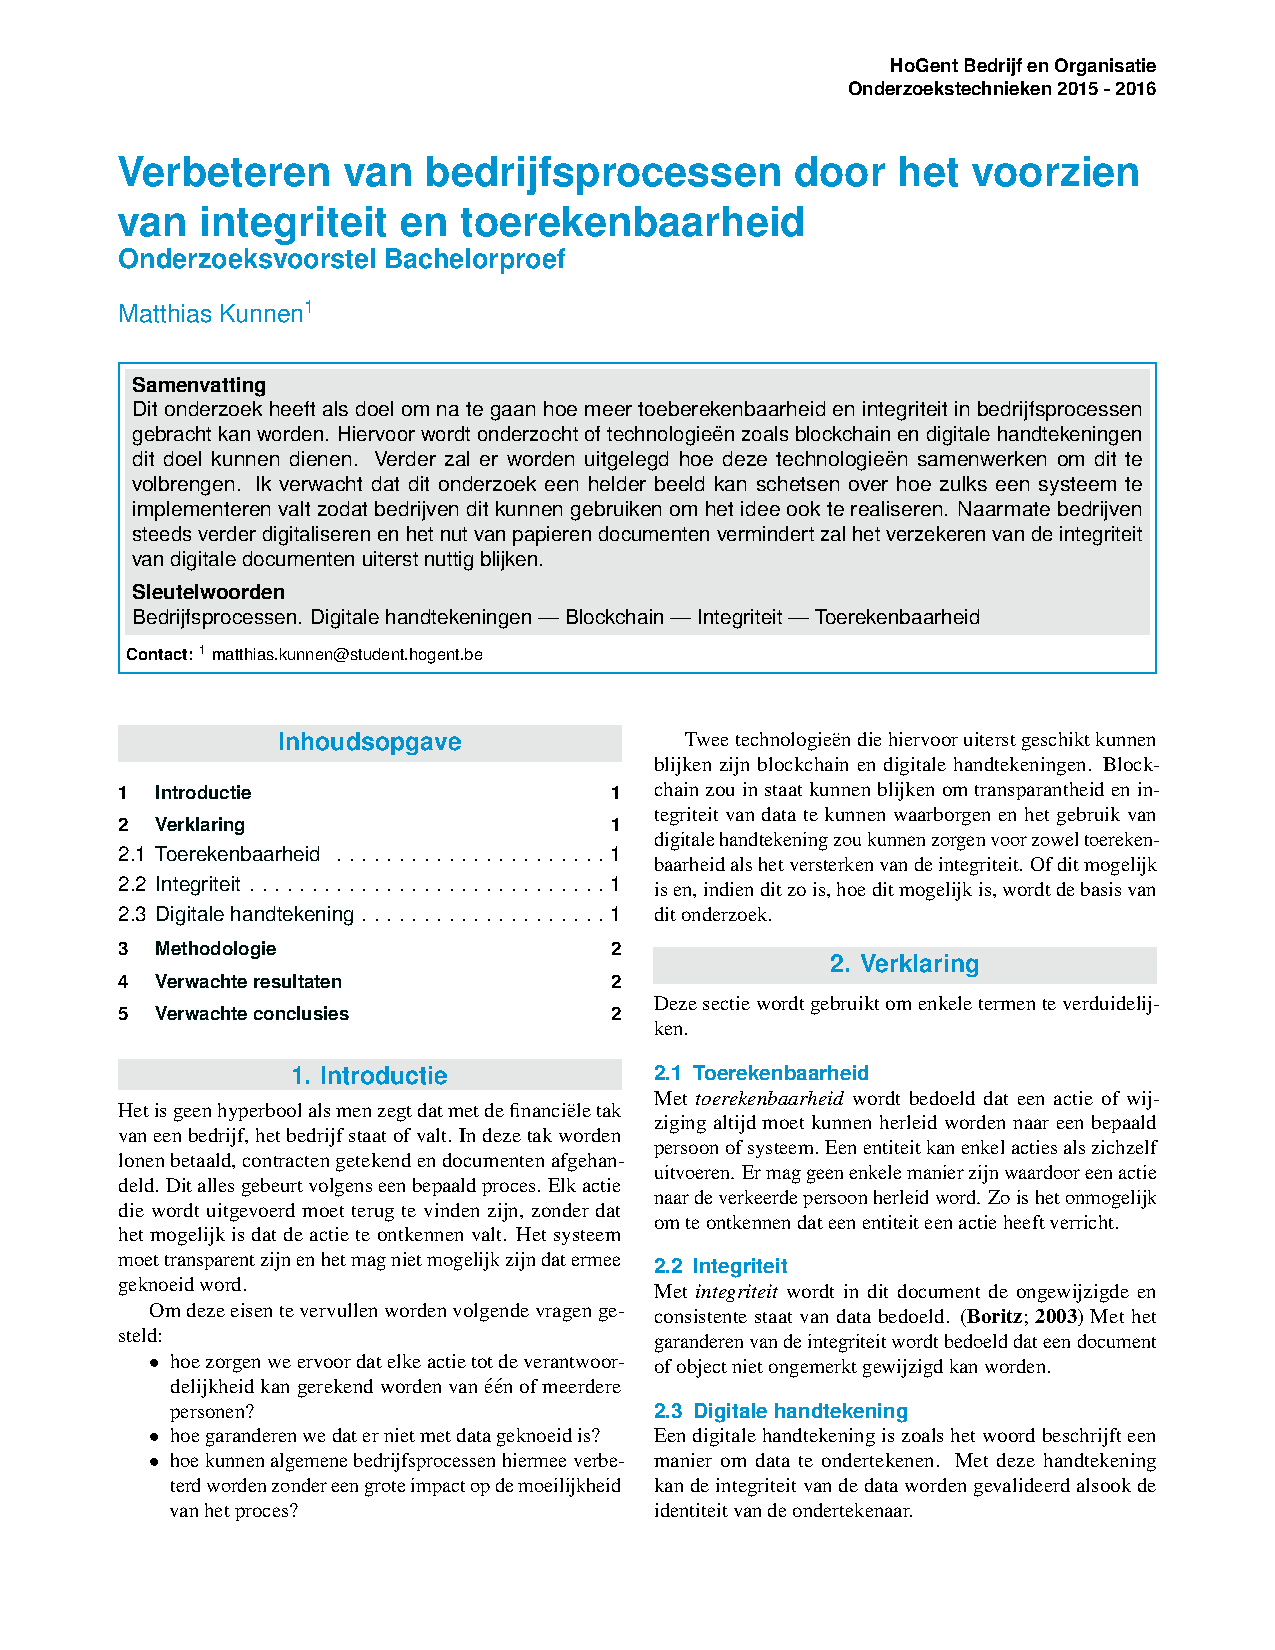
\includepdf[pages={-}]{kunnen-matthias-voorstel.pdf}
